% !TEX root = ../main.tex

\newlength\Radius
\setlength\Radius{2cm}

\section{Геометричні ймовірності. Аксіоми теорії ймовірностей.}
\subsection{Геометрична модель ймовірності}
\begin{example}
    Нехай точка кидається навмання на відрізок $\left[a, b\right]$. 
    Яка ймовірність її 
    потрапляння в $\left<\alpha, \beta\right> \subset  \left[a, b\right]$?
    \newline
    Розглянемо подію $A = \left\{ 
        \text{точка потрапила в} \left<\alpha, \beta\right>
    \right\}$.
    \newline
    \hbox to \hsize{\hfil{
        \begin{tikzpicture}
            \draw [fill] (0, 0) circle [radius = 0.05];
            \node [below] at (0, 0) {$a$};
            \node [above] at (0, 0) { };
            \node [below] at (8, 0) {$b$};
            \draw [-{Straight Barb}] (6,0) to (2,0) {};
            \draw [-{Straight Barb}] (2,0) to (6,0) {};
            \node [below] at (2, 0) {$\alpha$};
            \node [below] at (6, 0) {$\beta$};
            \draw [fill] (8, 0) circle [radius = 0.05];
            \draw [thick] (0, 0) -- (8, 0);
        \end{tikzpicture}
    }\hfil}
    $P(A) = kl_{\left<\alpha, \beta\right>}\; \text{для деякого}\; k > 0$.
    З іншого боку, $P(\Omega) = 1 = kl_{\left[a, b\right]}$. Таким чином 
    $k = \frac{1}{l_{\left[a, b\right]}} = \frac{1}{b-a}$.
    Тому $P(A) = \frac{l_{\left<\alpha, \beta\right>}}{l_{\left[a, b\right]}}$.
\end{example}
Нехай простір елементарних подій інтерпретується як замкнена область в 
$ \mathbb{R} ^n$, а випадкові події - її підмножини. В якості $\sigma-\text{алгебри}$ 
подій $\mathcal{F}$ беремо підмножини, що мають міру. Тоді в якості ймовірності 
деякої події $A$ беремо $P(A) = \frac{\mu(A)}{\mu(\Omega)}$
\newline
\hbox to \hsize{\hfil{
\begin{tabular}{ll}
    $\mathbb{R}^1$: & $P(A) = \dfrac{l_A}{l_\Omega}$ \\
    $\mathbb{R}^2$: & $P(A) = \dfrac{S_A}{S_\Omega}$ \\
    $\mathbb{R}^3$: & $P(A) = \dfrac{V_A}{V_\Omega}$ \\
\end{tabular}
}\hfil}
Ймовірності, що знаходяться таким чином називаються \emph{геометричними}, а сама модель 
називається \emph{геометричною моделлю ймовірності}.
\newline
Геометрична модель може використовуватись коли:
\begin{enumerate}
    \item $\Omega$ має геометричну інтерпретацію як замкнена область в $\mathbb{R}^n$.
    \item Елементарні події - рівноможливі.
\end{enumerate}
\begin{example}[Задача Бюффона]\label{buffon}
    На площині накреслені паралельні прямі на відстані $2a$, на них кидається 
    голка довжиною $2l,\; l \leq a $. Яка ймовірність того, що голка перетне 
    яку-небудь пряму?
    \newline
    \hbox to \hsize{\hfil{
        \begin{tikzpicture}[scale = 0.5]
            \draw [thick] (0, 0) -- (8, 0);
            \draw [thick] (0, 2) -- (8, 2);
            \draw [thick] (0, 4) -- (8, 4);
            \draw [thick] (0, 6) -- (8, 6);
            \draw [{Straight Barb}-{Straight Barb}] (7.5,4) to (7.5,6);
            \node [right] at (7.5, 5) {$2a$}; 
        \end{tikzpicture}
        \begin{tikzpicture}[scale = 1]
            \draw (0, 0) -- (4, 0);
            \draw (0, 2) -- (4, 2);
            \draw [thick] (0.5, -0.5)-- (2.5, 1.5);
            \draw [{Straight Barb}-{Straight Barb}] (3.5,0) to (3.5,2);
            \draw [{Straight Barb}-{Straight Barb}] (1.5,0) to (1.5,0.5);
            \node [right] at (3.5, 1) {$2a$};
            \node [right] at (1.5, 0.25) {$ x $};
            \draw [-{Straight Barb}](2.5, 0) to [out = 90, in = 0](1.75, 0.75);
            \node [right] at (2.28, 0.53) {$ \varphi $};
        \end{tikzpicture}
    }\hfil}
    Достатньо розглядати лише дві прямі. $\Omega = \left\{(\varphi, x)\in 
    \mathbb{R}^2: \varphi \in \left[0, \pi\right], x \in \left[0, \pi\right] 
    \right\}$
    \newline
    При такій побудові простору елементарних подій подія $A = \left\{\text{голка 
    перетне пряму}\right\} =$
    \newline
    $\left\{(\varphi, x)\in 
    \Omega: x\leq l\sin\varphi\right\}$
    \newline
    \hbox to \hsize{\hfil{
        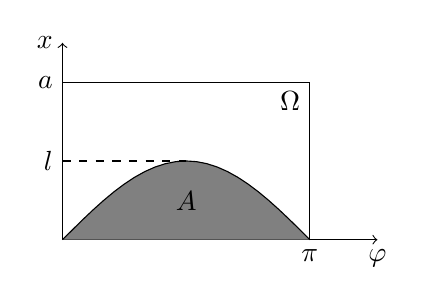
\begin{tikzpicture}
            \draw [<->] (4, 0) -- (0, 0) -- (0, 2.5);
            \node [left] at (0, 2.5) {$x$};
            \node [below] at (4, 0) {$\varphi$};
            \draw [domain=0:pi,fill=gray] plot (\x, {1*sin(\x r)});
            \node [below] at (pi, 0) {$\pi$};
            \draw [dashed] (0,1) to (pi/2,1);
            \node [left] at (0, 1) {$l$};
            \draw (0,2) -- (pi, 2) -- (pi, 0);
            \node [left] at (0, 2) {$a$};
            \node [below left] at (pi, 2) {$\Omega$};
            \node [above] at (pi/2, 0.25) {$A$};
        \end{tikzpicture}
    }\hfil}
    $P(A) = \frac{S(A)}{S(\Omega)},\; S(\Omega) = \pi a,\;S(A) = \int_0^\pi 
    l\sin\varphi\,\mathrm{d}x = l\left.(-\cos\varphi)\right|^\pi_0 = 2l$
    \newline
    Отже, $P(A) = \frac{2l}{\pi a}$.
    \newline
    Якщо провести $n$ кидань голки, з яких $m$ - кількість потраплянь голки 
    на пряму, то за допомогою приблизної рівності $\frac{m}{n} 
    \approx \frac{2l}{\pi a}$ можна приблизно обчислити число $\pi$.
\end{example}
\begin{example}[Парадокс Бертрана]
    Нехай в колі радіусом $r$ навмання проводиться хорда. Яка ймовірність того, 
    що довжина цієї хорди буде більшою за довжину сторони правильного трикутника, 
    що вписаний в це коло?
    \newline
    Існують три способи вирішення цієї задачі, при чому кожен з них дає різні 
    результати.
    \paragraph*{Спосіб 1}
    Виберемо випадково дві точки (A та B) на колі та проведемо через них хорду.
    Вписаний трикутник (без втрати загальності) 
    будуємо так, щоб його вершина лежала у першій вибраній точці. Друга вибрана на колі 
    точка однозначно визначає хорду; таким чином кожну з хорд можна співставити з 
    деякою точкою на колі. 
    \newline
    \hbox to \hsize{\hfil{
        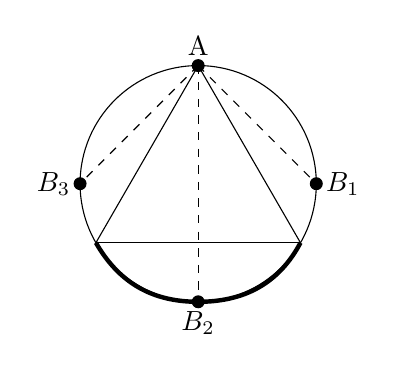
\begin{tikzpicture}[scale = 1.5]
            \draw (0, 0) circle [radius = 1];
            \draw (0, 1) -- (-0.86602540378, -0.5); 
            \draw (0, 1) -- (0.86602540378, -0.5);
            \draw (0.86602540378, -0.5) -- (-0.86602540378, -0.5);
            \draw [fill] (0, 1) circle [radius = 0.05];
            \draw [fill] (0, -1) circle [radius = 0.05];
            \draw [fill] (1, 0) circle [radius = 0.05];
            \draw [fill] (-1, 0) circle [radius = 0.05];
            \node [above] at (0, 1) {A};
            \draw [dashed] (0,1) to (0, -1);
            \draw [dashed] (0,1) to (1, 0);
            \draw [dashed] (0,1) to (-1, 0);
            \node [right] at (1, 0) {$B_1$};
            \node [below] at (0, -1) {$B_2$};
            \node [left] at (-1, 0) {$B_3$};
            \draw [ultra thick](0.86602540378, -0.5) to [out = 242, in = 0](0, -1);
            \draw [ultra thick](0, -1) to [out = 180, in = 300](-0.86602540378, -0.5);
        \end{tikzpicture}
    }\hfil}
    $\Omega = \left[0, 2\pi r\right).$ Можна побачити, що якщо точка B потрапить 
    в нижню третину кола, то хорда буде довшою за сторону трикутника. Таким чином 
    подію T = \{довжина хорди більше ніж довжина сторони трикутника\} 
    можна інтерпретувати геометрично як $T = [\frac{2}{3}\pi r, \frac{4}{3}\pi r]$.
    Згідно з геометричної схеми, $P(T) = \frac{l_T}{l_\Omega} = \frac{1}{3}$.
    \paragraph*{Спосіб 2}
    Для будь-якої хорди маємо радіус, що проходить через середину цієї хорди 
    перпендикулярно їй. Без 
    втрати загальності "повернемо" вписаний трикутник так, щоб його ближча сторона 
    була паралельна хорді. Сторона трикутника розділює обраний радіус на дві половини. 
    Таким чином можна співставити кожну хорду з деякою точкою на радіусі. Якщо точка 
    буде лежати на половині радіуса "ззовні" вписаного трикутника, то відповідна хорда 
    буде коротше за сторону трикутника, в іншому випадку - довше. Таким чином маємо 
    геометричну інтерпретацію для простору елементарних подій та нашої події, ймовірність 
    якої ми шукаємо.
    \newline
    \hbox to \hsize{\hfil{
        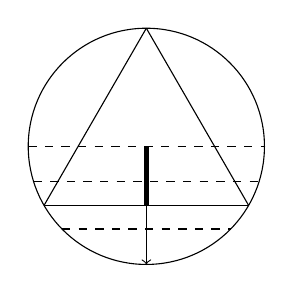
\begin{tikzpicture}[scale = 1.5]
            \draw (0, 0) circle [radius = 1]; 
            \draw (0, 1) -- (-0.86602540378, -0.5); 
            \draw (0, 1) -- (0.86602540378, -0.5);
            \draw (0.86602540378, -0.5) -- (-0.86602540378, -0.5);
            %\draw [fill] (0, 1) circle [radius = 0.05];
            \draw [->] (0,0) to (0, -1);
            \draw [dashed] (-1, 0) to (1, 0);
            \draw [dashed] (-0.954, -0.3) to (0.954, -0.3);
            \draw [dashed] (-0.714, -0.7) to (0.714, -0.7);
            \draw [ultra thick] (0, 0) -- (0, -0.5);
        \end{tikzpicture}
    }\hfil}
    $\Omega = [0, r], T = [0, \frac{r}{2}], P(T) = \frac{l_T}{l_\Omega} = \frac{1}{2}$.
    \paragraph*{Спосіб 3}
    цввввввв
    \newline
    \hbox to \hsize{\hfil{
        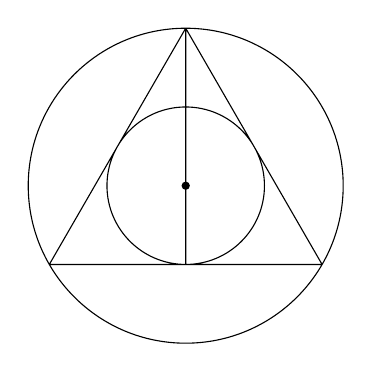
\begin{tikzpicture}[line join=round]
            \draw 
              (0,0) circle [fill = gray, radius=\Radius]
              (0,0) circle [radius=0.5\Radius]
              (90:\Radius) -- (210:\Radius) -- (-30:\Radius) -- cycle
              %(0,0) -- (210:\Radius) node[midway,above] {$R$}
              %(0,0) -- (-30:0.5\Radius) node[midway,above] {$r$}
              (90:\Radius) -- (90:-0.5\Radius);
            \fill (0,0) circle [radius=1.5pt];
            \end{tikzpicture}
    }\hfil}
\end{example}